Sei \(k\) gerade und \(\mathcal{M}^{2k}\) eine \(4m\)-dimensionale \(\pi\)-Mannigfaltigkeit. Dann existiert eine \textit{topologische} Kobordismus-Invariante die genutzt werden kann um zu entscheiden ob eine Chirurgie an einer \(k\)-Sph\"are die Homologie vereinfacht. Zudem existiert mit Satz \ref{thm:intersect_even} eine relativ einfache Methode um zu entscheiden, wann das Normalenb\"undel einer eingebetteten Sph\"are trivial ist. In Folge dessen, ist es relativ einfach \(P_{4m}\) zu berechnen. Im Gegensatz dazu steht die Berechnung von \(\partial P_{4m}\), die sich als deutlich aufw\"andiger erweist, und einige Kenntnisse zu \textit{fast parallelisierbaren} Mannigfaltigkeiten ben\"otigt. Die Anzahl der Elemente in \(\partial P^{4k}\) ist gerade
\[2^{2k-3}\left(2^{2k-1}-1\right)\left(3+(-1)^{k+1}\right)\,\text{\upshape Z\"ahler}\left(\frac{B_{2k}}{4k}\right)\,,\]
Dieser zun\"achst kurios erscheinende Term setzt sich aus einigen unterschiedlichen Ausdr\"ucken zusammen, wie zum Beispiel den Koeffizienten der Potenzreihe
\[\frac{\sqrt{t}}{\sinh\left(2\sqrt{t}\right)}=\sum_{k\geq0}\frac{2^{2k}(2^{2k-1}-1)B_{2k}}{(2k)!}t^k\]
und dem Rang des Bildes des \(J\)-Homomorphismus
\[\operatorname{Rang}\operatorname{Im}J_{4k-1}=\,\text{Nenner}\left(\frac{B_{2k}}{4k}\right)\,.\]
\newpage
\section{Die Schnittpaarung in vierfacher Dimension}
    Zun\"achst ist es vonn\"oten zu entscheiden, wann das Normalenb\"undel \(\nu\) einer in eine eingebetteten Sph\"are nicht nur stabil trivial, sondern bereits trivial ist. Da \(\nu\) stabil trivial ist, liegt es in \(\ker S_*\). Betrachte hierzu zun\"achst die Abbildung
\[\Phi\colon\ker S_*\to\mathbb{Z}\,,\eqcl{\xi}\mapsto\left\langle e\left(\xi\right),\eqcl{\mathbb{S}^k}\right\rangle\,.\]
Aus den Eigenschaften der Euler-Klasse folgt, dass dies ein wohldefinierter Homomorphismus ist. Dieser ist jedoch f\"ur ungerade \(k\) trivial, da in diesem Fall \(\ker S_*\cong\mathbb{Z}_2\) endlich ist.
\begin{lemma}\label{lem:phi_mono_even}
    F\"ur gerade \(k\) ist \(\Phi\) ein Monomorphismus, der lediglich gerade Werte annimmt.
\end{lemma}
\begin{proof}
    Der Kern \(\ker S_*\) wird von \(\eqcl{\tau_k}\) erzeugt, und ist, da \(k\) gerade ist, zyklisch unendlich. Folglich ist jedes \(\eqcl{\xi}\in\ker S_*\) ein Vielfaches von \(\eqcl{\tau_k}\), sei etwa \({\eqcl{\xi}=\beta\cdot\eqcl{\tau_k}}\). Da die Euler-Klasse von \(\tau_k\) das Doppelte eines Erzeugers \(g\in H^k(\mathbb{S}^k)\) ist (Siehe \cite{hatcher2017vector} Proposition 3.14), gilt
    \[\Phi(\eqcl{\xi})=\left\langle e(\xi),\eqcl{\mathbb{S}^k}\right\rangle=2\beta\cdot\left\langle g,\eqcl{\mathbb{S}^k}\right\rangle\,.\]
    Da \(\langle g,\eqcl{\mathbb{S}^k}\rangle\not=0\) ist, ist dies genau dann null, wenn \(\beta=0\), und somit \(\eqcl{\xi}=0\) ist.
\end{proof}
Sei \(\mathcal{M}^{2k}\) eine \(\pi\)-Mannigfaltigkeit, und \(\mathcal{S}^k\hookrightarrow\mathring{\mathcal{M}}\) eine eingebettete Sph\"are. Dann folgt aus dem vorangegangenen Lemma, dass das Normalenb\"undel \(\nu\) von \(\mathcal{S}\) genau dann trivial ist, wenn \(\Phi(\nu)=0\) gilt. Um dies zu entscheiden ist das folgende Lemma hilfreich.
\begin{lemma}\label{lem:euler_dual}
    Sei \(\mathcal{M}^{i+j}\) eine orientierte Mannigfaltigkeit und \(\iota\colon\mathcal{V}^i\hookrightarrow\mathring{\mathcal{M}}\) eine geschlossene Untermannigfaltigkeit mit Normalenb\"undel \(\nu\). Dann gilt
    \begin{equation}\label{eq:euler_dual}
        e(\nu)=\pm\iota^*q^*\eqcl{\mathcal{V}\mathrel{|}\mathcal{M}}^*\quad\text{also}\quad\langle e(\nu),\eqcl{\mathcal{V}}\rangle=\pm\eqcl{\mathcal{V}\mathrel{|}\mathcal{M}}\cdot\eqcl{\mathcal{V}\mathrel{|}\mathcal{M}}\,.
    \end{equation}
\end{lemma}
\begin{proof}
    Sei \(\mathcal{D}\subseteq\mathring{\mathcal{M}}\) eine geschlossene Tubenumgebung von \(\mathcal{V}\). Betrachte die kanonischen Inklusionen
    \[d\colon(\mathcal{D},\partial\mathcal{D})\hookrightarrow\big(\mathcal{M},\mathcal{M}\setminus\mathring{\mathcal{D}}\big)\quad\text{und}\quad f\colon(\mathcal{M},\partial\mathcal{M})\hookrightarrow\big(\mathcal{M},\mathcal{M}\setminus\mathring{\mathcal{D}}\big)\,.\]
    Sei \(X:=f_*\eqcl{\mathcal{M}}=d_*\eqcl{\mathcal{D}}\). Dann kommutiert das Diagramm
    \begin{center}
        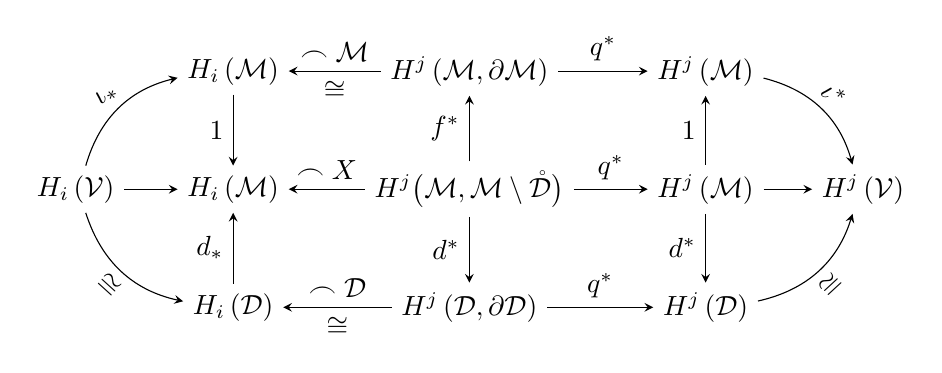
\begin{tikzpicture}
            \draw
                (0, 0) node (A) {\(H_i\left(\mathcal{V}\right)\)}
                (2, -1.5) node (B) {\(H_i\left(\mathcal{D}\right)\)}
                (2, 0) node (C) {\(H_i\left(\mathcal{M}\right)\)}
                (2, 1.5) node (D) {\(H_i\left(\mathcal{M}\right)\)}
                (5, -1.5) node (E) {\(H^j\left(\mathcal{D},\partial\mathcal{D}\right)\)}
                (5, 0) node (F) {\(H^j\big(\mathcal{M},\mathcal{M}\setminus\mathring{\mathcal{D}}\big)\)}
                (5, 1.5) node (G) {\(H^j\left(\mathcal{M},\partial\mathcal{M}\right)\)}
                (8, -1.5) node (H) {\(H^j\left(\mathcal{D}\right)\)}
                (8, 0) node (I) {\(H^j\left(\mathcal{M}\right)\)}
                (8, 1.5) node (J) {\(H^j\left(\mathcal{M}\right)\)}
                (10, 0) node (K) {\(H^j\left(\mathcal{V}\right)\)}

                (A) edge [-stealth, bend right] node [sloped, below] {\(\cong\)} (B)
                (A) edge [-stealth] (C)
                (A) edge [-stealth, bend left] node [sloped, above] {\(\iota_*\)} (D)
                
                (E) edge [-stealth] node [below] {\(\cong\)} node [above] {\(\frown\eqcl{\mathcal{D}}\)} (B)
                (E) edge [-stealth] node [above] {\(q^*\)} (H)
                (H) edge [-stealth, bend right] node [sloped, below] {\(\cong\)} (K)
                
                (F) edge [-stealth] node [above] {\(\frown X\)} (C)
                (F) edge [-stealth] node [above] {\(q^*\)} (I)
                (I) edge [-stealth] (K)

                (G) edge [-stealth] node [below] {\(\cong\)} node [above] {\(\frown\eqcl{\mathcal{M}}\)} (D)
                (G) edge [-stealth] node [above] {\(q^*\)} (J)
                (J) edge [-stealth, bend left] node [sloped, above] {\(\iota^*\)}  (K)
                
                (B) edge [-stealth] node [left] {\(d_*\)} (C)
                (D) edge [-stealth] node [left] {\(\mathbbm{1}\)} (C)
                
                (F) edge [-stealth] node [left] {\(d^*\)} (E)
                (F) edge [-stealth] node [left] {\(f^*\)} (G)
                
                (I) edge [-stealth] node [left] {\(d^*\)} (H)
                (I) edge [-stealth] node [left] {\(\mathbbm{1}\)} (J)
                ;
        \end{tikzpicture}
    \end{center}
    Hierbei korrespondiert ein Generator von \(H^j\left(\mathcal{D},\partial\mathcal{D}\right)\) mit der Thom-Klasse von \(\nu\), und wird deshalb in \(H^j(\mathcal{V})\) auf die Euler-Klasse von \(\nu\) abgebildet. Durch eine Jagd der Fundamentalklasse \(\eqcl{\mathcal{V}}\in H_i(\mathcal{V})\) durch die obere und untere Zeile ergibt sich
    \[\pm\iota^*q^*\eqcl{\mathcal{V}\mathrel{|}\mathcal{M}}^*=e(\nu)\,.\]
    Es gilt also
    \begin{align*}
        \mp\left\langle e(\nu),\eqcl{\mathcal{S}}\right\rangle&=\left\langle\iota^*q^*\eqcl{\mathcal{S}\mathrel{|}\mathcal{M}}^*,\eqcl{\mathcal{S}}\right\rangle\\
        &=\left\langle q^*\eqcl{\mathcal{S}\mathrel{|}\mathcal{M}}^*,\eqcl{\mathcal{S}\mathrel{|}\mathcal{M}}\right\rangle\mathop{=}^{\text{\tiny\eqref{eq:intersect_prop_2}}}\eqcl{\mathcal{S}\mathrel{|}\mathcal{M}}\cdot\eqcl{\mathcal{S}\mathrel{|}\mathcal{M}}\,.
    \end{align*}
\end{proof}
Der Beweis orientiert sich an einem \"ahnlichen Lemma aus Lecture 11 von \cite{auroux2012algebraic}.

\begin{theorem}\label{thm:intersect_even}
    Sei \(k\geq3\) gerade und \(\mathcal{M}^{2k}\) eine \((k-1)\)-zusammenh\"angende \(\pi\)-Mannig\-faltig\-keit. Dann ist die Schnittpaarung gerade, und es gilt \({x\cdot x=0}\) genau dann, wenn \({\alpha(x)=0}\) ist.
\end{theorem}
\begin{proof}
    Zun\"achst gilt \(\alpha(x)\in\ker S_*\) gem\"a\ss{} Gleichung \ref{eq:alpha_kernel}. Sei \({\iota\colon\mathcal{S}\hookrightarrow\mathring{\mathcal{M}}}\) eine \(x\) repr\"asentierende Einbettung mit Normalenb\"undel \(\nu\). Dann gelten per Definitionem
    \(x=\eqcl{\mathcal{S}\mathrel{|}\mathcal{M}}\) und \(\alpha(x)=\eqcl{\nu}\). Zusammen ergibt dies
    \[x\cdot x=\eqcl{\mathcal{S}\mathrel{|}\mathcal{M}}\cdot\eqcl{\mathcal{S}\mathrel{|}\mathcal{M}}\mathop{=}^{\text{\tiny\eqref{eq:euler_dual}}}\mp\left\langle e(\nu),\eqcl{\mathcal{S}}\right\rangle=\mp\Phi(\alpha(x))\,.\]
    Dann ist die Aussage des Satzes eine direkte Konsequenz von Lemma \ref{lem:phi_mono_even}.
\end{proof}


\section{Die Signatur}
    Da \(k\) gerade und die Schnittform symmetrisch ist, kann diese \"uber \(\mathbb{R}\) diagonalisiert werden. Sei \(n_+\) die Anzahl der positiven und \(n_-\) die Anzahl der negativen Eintr\"age einer Diagonalisierung. Die \textbf{Signatur} von \(\mathcal{M}\) sei definiert als \(\sigma(\mathcal{M}):=n_+-n_-\). F\"ur ungerade \(k\), also wenn die Schnittform schiefsymmetrisch ist, sind alle Eigenwerte komplex, sodass keine Diagonalisierung \"uber \(\mathbb{R}\) existieren kann. 
\begin{theorem}\label{thm:sign_prop}
    F\"ur kompakte, orientierte topologische Mannigfaltigkeiten \(\mathcal{M}^n\), \(\mathcal{N}^n\) gilt
    \begin{itemize}
        \item[i] F\"ur eine Mannigfaltigkeit \(\mathcal{W}^{4m+1}\) gilt \(\sigma(\partial\mathcal{W})=0\)
        \item[ii] \(\sigma(\mathcal{M}\sqcup\mathcal{N})=\sigma(\mathcal{M}+\mathcal{N})=\sigma(\mathcal{M})+\sigma(\mathcal{N})\)
        \item[iii] Es gilt \(\sigma(\mathcal{M}\times\mathcal{N})=\sigma(\mathcal{M})\sigma(\mathcal{N})\)
        \item[iv] Die Signatur einer geraden, unimodularen Form teilt acht
    \end{itemize}
\end{theorem}
\begin{proof}
    \subsubsection{Behauptung \(i\)}
        Aus Gleichung \ref{eq:ker_incl_dim} folgt
        \[2\dim_{\mathbb{R}}\ker\iota_*=\dim_{\mathbb{R}}H_k(\partial\mathcal{W};\mathbb{R})\,.\]
        Weiter verschwindet \(Q(x):=x\cdot x\) auf \(\ker\iota_*\), also folgt
        \[\abs{\sigma(\partial\mathcal{W})}=\abs{\sigma(Q)}\leq\dim_{\mathbb{R}}H_k(\partial\mathcal{W};\mathbb{R})-2\dim_{\mathbb{R}}\ker\iota_*=0\]
        und somit \(\sigma(\partial\mathcal{W})=0\).
    \subsubsection{Behauptung \(ii\)}
        Das folgt, da die mittlere Homologiegruppe der disjunkten Vereinigung, der verbundene Summe und der verbundene Randsumme spaltet, und somit zu \(H_k(\mathcal{M})\oplus H_k(\mathcal{N})\) isomorph ist.
\end{proof}
Der Beweis von \(i\) folgt \cite{dold1980lectures} Proposition 9.6. F\"ur einen Beweis von iii siehe \cite{tomdieck2008algebraic} Proposition 18.7.3. Obwohl Satz \ref{thm:sign_prop} keine glatte Struktur fordert folgt aus ihr nur, dass die Signatur eine Chirurgie-Invariante f\"ur geschlossene Mannigfaltigkeiten ist. Ist \(\mathcal{M}\) eine Mannigfaltigkeit mit nicht-leerem Rand, ist \(\mathcal{M}\times\mathbb{I}\) zwar erneut eine Mannigfaltigkeit mit Rand, jedoch gilt
\[\partial\left(\mathcal{M}\times\mathbb{I}\right)=\partial\mathcal{M}\times\mathbb{I}\cup\mathcal{M}\times\partial\,\mathbb{I}\,.\]

\begin{lemma}\label{lem:4n_symp}
    Eine freie abelsche Gruppe mit einer unimodularen, geraden quadratischen Form \(\beta\) mit Signatur null besitzt eine schwach symplektische Basis.
\end{lemma}
\begin{proof}
    Da die Signatur null ist, ist die Form indefinit, und besitzt gem\"a\ss{} \cite{milnor1961procedure} Lemma 8 eine nicht-triviale Nullstelle \(e_1\). Da die Form unimodular ist, existiert ein \(\alpha\in H_k(\mathcal{M})\) mit \(\beta(\alpha,e_1)=1\). Da sie gerade ist, l\"asst sich
    \[f_1:=\alpha-\frac{\beta(\alpha,\alpha)}{2}e_1\]
    definieren. Es folgen
    \[\beta(e_1,f_1)=\beta(e_1,\alpha)-\frac{\beta(\alpha,\alpha)}{2}\beta(e_1,e_1)=1\]
    und
    \[\beta(f_1,f_1)=\beta(\alpha,\alpha)-\frac{2\beta(\alpha,\alpha)}{2}\beta(\alpha,e_1)+0=0\,.\]
    Aus der Unimodularit\"at folgt weiter, dass \(H\) in die direkte Summe der Untergruppe \(\langle e_1,f_1\rangle\) und des orthogonalen Komplements spaltet. Die Aussage folgt \"uber eine Induktion \"uber den Rang der Gruppe.
\end{proof}
\newpage
\begin{theorem}\label{thm:sign_inv}
    Die Signatur induziert einen Monomorphismus \(\sigma\colon P^{4m}\to\mathbb{Z}\).
\end{theorem}
\begin{proof}
    \subsubsection*{Wohldefiniertheit}
        Sei \({n=i+j+1}\). Es reicht aus \({\sigma(\mathcal{M})=\sigma(\mathcal{N})}\) f\"ur \({\mathcal{N}=\mathcal{M}\multimap\mathbb{S}^i}\) zu zeigen. Es kann zudem angenommen werden, dass \(i\leq j\) gilt, denn l\"asst sich \(\mathcal{N}\) durch gerahmte \(i\)-Chirurgie aus \(\mathcal{M}\) erhalten, l\"asst sich \(\mathcal{M}\) durch gerahmte \(j\)-Chirurgie aus \(\mathcal{N}\) erhalten. Gem\"a\ss{} Lemma \ref{lem:smoothing_pi} existiert eine gerahmte Mannigfaltigkeit \(\mathcal{W}^{n+1}\) mit 
        \[\partial\mathcal{W}\cong\mathcal{M}\mathop{+}^{\partial\mathcal{M}}\mathcal{N}\,.\]
        Aus Proposition \ref{thm:sign_prop} folgt \(\sigma(\partial\mathcal{W})=0\), da \(\partial\mathcal{M}\) eine Homotopiesph\"are ist, ist weiter
        \[H_k(\partial\mathcal{W})\cong H_k(\mathcal{M})\oplus H_k(\mathcal{N})\,,\]
        also \(0=\sigma(\partial\mathcal{W})=\sigma(\mathcal{M})-\sigma(\mathcal{N})\) und somit \(\sigma(\mathcal{M})=\sigma(\mathcal{N})\). 

    \subsubsection*{Injektivit\"at}
        Sei \(k\) gerade und \((\mathcal{M}^{2k},F)\) eine gerahmte Mannigfaltigkeit in \(\ker\sigma\). Da \(\partial\mathcal{M}\) eine Homotopiesph\"are ist, ist \(H_k(\mathcal{M})\) gem\"a\ss{} Lemma \ref{lem:middle_free} frei. Da die Schnittform symmetrisch, gerade \ref{thm:intersect_even} und unimodular \ref{crl:intersect_uni} ist und \(\sigma(\mathcal{M})=0\) gilt, besitzt \(H_k(\mathcal{M})\) gem\"a\ss{} Satz \ref{lem:4n_symp} eine schwach symplektische Basis \(e_i,f_i\) mit
        \[e_i\cdot e_j=f_i\cdot f_j=0\quad\text{und}\quad e_i\cdot f_j=\delta_{ij}\,.\]
        Aus Satz \ref{thm:intersect_even} folgt, dass \({\alpha(e_i)=0}\) gilt, sodass \(\mathcal{M}\) gem\"a\ss{} Satz \ref{thm:even_symp_ann} zu einer \(k\)-zusammenh\"angenden gerahmten Mannigfaltigkeit \(\chi\)-\"aquivalent ist und damit das triviale Element in \(P_{4m}\) repr\"asentiert. Die Homomorphismus-Eigenschaft folgt aus Lemma \ref{thm:sign_prop}.
\end{proof}

\begin{example}[Milnor-Mannigfaltigkeit]\label{ex:milnor_man}
    Es existiert eine \(4n\)-Mannigfaltigkeit \(M(4n)\), deren Schnittform durch die Matrix
    \[\Gamma_8:=\begin{pmatrix}
        2 & 1 & 0 & 0 & 0 & 0 & 0 & 0\\
        1 & 2 & 1 & 0 & 0 & 0 & 0 & 0\\
        0 & 1 & 2 & 1 & 0 & 0 & 0 & 0\\
        0 & 0 & 1 & 2 & 1 & 0 & 0 & 0\\
        0 & 0 & 0 & 1 & 2 & 1 & \mathcolor{red}{1} & 0\\
        0 & 0 & 0 & 0 & 1 & 2 & \mathcolor{red}{0} & 0\\
        0 & 0 & 0 & 0 & \mathcolor{red}{1} & \mathcolor{red}{0} & 2 & 1\\
        0 & 0 & 0 & 0 & 0 & 0 & 1 & 2
    \end{pmatrix}\]
    gegeben ist. Durch eine Rechnung folgt \(\det(\Gamma_8)=1\) und \(\sigma(\Gamma_8)=8\). Es gilt also \(\sigma(M(4n))=8\). Diese l\"asst sich konstruieren, indem an eine \(2k\)-Scheibe acht \(k\)-Henkel angebracht werden. Hierzu werden disjunkte Anklebeabbildungen \(\phi_i\colon\mathbb{S}^{k-1}\hookrightarrow\mathbb{D}^{2k}\), die sich f\"ur \(k\geq3\) zu disjunkten eingebetteten Scheiben fortsetzen lassen. In der Mannigfaltigkeit \(\mathcal{D}\), welche durch das Anbringen von Henkeln entlang der \(\phi\) entsteht, k\"onnen nun diese eingebetteten Scheiben als untere-, und die Kerne der Henkel als obere Hemisph\"aren aufgefasst werden. F\"ur jeden Henkel ergibt sich derart eine \(k\)-Sph\"are. Es l\"asst sich zeigen, dass sich die Anklebeabbildungen derart w\"ahlen lassen, dass zu gegebenen Elementen \(\eqcl{\gamma_i}\in\pi_{k-1}\left(\operatorname{SO}\left(k\right)\right)\) die Kupplungsfunktionen der Normalenb\"undel der Pr\"asentationssph\"aren gerade die \(\gamma_i\) sind. Wird nun acht mal \(\tau_k\) gew\"ahlt, ergibt sich die Milnor-Mannigfaltigkeit. Die Schnittform wird durch die Matrix \(\Gamma_8\) beschrieben, dass zugeh\"orige Gitter ist durch das au\ss erordentliche Dynkin-Diagramm \(E_8\) klassifiziert.
    \begin{figure}[!ht]
        \centering
        \begin{tikzpicture}
            \draw 
                (1, 0) node [state, minimum size = 5pt] (A) {}
                (2, 0) node [state, minimum size = 5pt] (B) {}
                (3, 0) node [state, minimum size = 5pt] (C) {}
                (4, 0) node [state, minimum size = 5pt] (D) {}
                (5, 0) node [state, minimum size = 5pt] (E) {}
                (5, 1) node [state, minimum size = 5pt] (F) {}
                (6, 0) node [state, minimum size = 5pt] (G) {}
                (7, 0) node [state, minimum size = 5pt] (H) {}

                (A) -- (B) -- (C) -- (D) -- (E) -- (G) -- (H)
                (F) -- (E)
            
            ;
        \end{tikzpicture}
    \end{figure}
\end{example}

\begin{theorem}\label{thm:sign_image}
    Es gilt \(P^{4m}\cong\operatorname{Im}\sigma=8\mathbb{Z}\).
\end{theorem}
\begin{proof}
    Sei \((\mathcal{M},F)\in P^{4m}\). Dann ist \(\sigma(\mathcal{M})\) gem\"a\ss{} \ref{thm:sign_prop} durch acht teilbar. Da \(\sigma\) gem\"a\ss{} \ref{thm:sign_inv} ein Monomorphismus ist, ist \(P^{4m}\) zu einer Untergruppe von \(8\mathbb{Z}\) isomorph. Die Aussage folgt, da die Milnor-Mannigfaltigkeit \(M(4m)\) in \(P^{4m}\) liegt und Signatur \(8\) besitzt \ref{ex:milnor_man}.
\end{proof}

\section{Der Signatursatz von Hirzebruch}
    Ein wichtiger Satz, welcher f\"ur die Berechnung von \(P_{4k}\) ben\"otigt wird, ist der Signatursatz von Hirzebruch. Er besagt, dass ein bestimmtes Polynom \(L_k\) existiert, sodass sich die Signatur durch die Pontrjagin-Klassen des Tangential\-b\"un\-dels \(p_i\) wie folgt darstellen l\"asst:
\[\sigma(\mathcal{M})=\langle L_k(p_1,\dots,p_k),\eqcl{\mathcal{M}}\rangle\,.\]
Um diese \(L\)-Polynome zu definieren, ist etwas Kombinatorik vonn\"oten. Das Folgende sei nur ein kurzer Anriss der eigentlichen Thematik, f\"ur eine pr\"azisere Abhandlung des Satzes siehe zum Beispiel \cite{milnor1974characteristic} \S19. 

\subsection{Multiplikative Folgen}
    Eine Folge \(K_i\in\Lambda\eqcl{X_1,\dots,X_i}\) homogener Polynome \(i\)-ten Grades hei\ss e multiplikativ, wenn \(K_0=1\) ist und f\"ur alle formalen Potenzreihen \(a,b,c\in\Lambda[[t]]\) mit Leitkoeffizient \(1\) und \(c=ab\) die Gleichung
    \[\sum_{i\geq0}K_i(c_1,\dots,c_i)t^i=\bigg(\sum_{i\geq0}K_i(a_1,\dots,a_i)t^i\bigg)\bigg(\sum_{i\geq0}K_i(b_1,\dots,b_i)t^i\bigg)\,,\]
    gilt. Schreibe auch \(K(ab)=K(a)K(b)\). Zu jeder multiplikativen Folge geh\"ort nun die \textbf{charakteristische Potenzreihe} \(K(1+t)\in\Lambda[[t]]\). Dass die Korrespondenz von multiplikativen Folge zu ihren charakteristischen Potenzreihen bijektiv ist, ist durch folgenden Satz gegeben.
    \begin{proposition}
        Zu jeder Potenzreihe \(f\in\Lambda[[t]]\) existiert genau eine multiplikative Folge \(K_i\) mit \(K(1+t)=f(t)\).
    \end{proposition}
    Die zu der Potenzreihe
    \[\frac{\sqrt{x}}{\tanh(\sqrt{x})}=\sum_{k\geq0}\frac{2^{2k}B_{2k}}{(2k)!}x^k\]
    geh\"orende Folge sei im Folgenden mit \(L_k\) bezeichnet, f\"ur eine \(4k\)-di\-men\-sio\-na\-le geschlossene und orientierte Manngifaltigkeit sei
    \[\mathcal{L}(\mathcal{M}):=\langle L_k(p_1,\dots,p_k),\eqcl{\mathcal{M}}\rangle\]
    der \textbf{L-Genus}, wobei \(p_j\) die \(j\)-te Pontrjagin-Klasse von \(T\mathcal{M}\) bezeichne. Die Wahl der charakteristischen Potenzreihe wirkt zun\"achst etwas willk\"urlich, kann jedoch als Normalisierung verstanden werden. Durch sie kann
    \[\mathcal{L}\left(\mathbb{C}P^{2m}\right)=1\]
    garantiert werden.

    \subsubsection{Der orientierte Kobordismusring}
        Zusammen mit der disjunkten Vereinigung bildet die Menge der orientierten Kobordismusklassen orientierter geschlossener Mannigfaltigkeiten \(\Omega_k^{\text{\tiny Or}}\) eine abelsche Gruppe. Diese wird von den Produkten \(\mathbb{C}P^{2n_1}\times\dots\times\mathbb{C}P^{2n_{\ell}}\) f\"ur alle Zerlegungen \(\sum n_i=k\) erzeugt. Dann erh\"alt
        \[\Omega_*^{\text{\tiny Or}}:=\bigoplus_{k\geq0}\Omega_{4k}^{\text{\tiny Or}}\,.\]
        mithilfe des kartesischen Produkts die Struktur eines graduierten Ringes. Insbesondere bilden die \(\mathbb{C}P^{2k}\) eine Basis des torsionsbefreiten Kobordismusrings \(\Omega_*^{\text{\tiny Or}}\otimes\mathbb{Q}\).
    \begin{proposition}
        Die Abbildung \(\mathcal{L}\colon\Omega_*^{\text{\tiny Or}}\otimes\mathbb{Q}\to\mathbb{Q},\,\mathcal{M}\mapsto\mathcal{L}\left(\mathcal{M}\right)\) ist ein Ringhomomorphismus.
    \end{proposition}
    Der Signatursatz von Hirzebruch ist nun eine direkte Konsequenz aus dem vorangegangenen Satz. Sowohl \(\sigma\) als auch \(\mathcal{L}\) definieren Ringhomomorphismen \(\Omega_*^{\text{\tiny Or}}\otimes\mathbb{Q}\to\mathbb{Q}\), und auf der Menge der Generatoren \(\mathbb{C}P^{2k}\) gilt
    \[\sigma\left(\mathbb{C}P^{2k}\right)=1=\mathcal{L}\left(\mathbb{C}P^{2k}\right)\,.\]
    Dies zeigt:
    \begin{proposition}[Signatursatz von Hirzebruch]\label{prop:signature_thm}
        Die Signatur \(\sigma(\mathcal{M})\) einer geschlossenen Mannigfaltigkeit \(\mathcal{M}\) ist gleich dem L-Genus \(\mathcal{L}(\mathcal{M})\).
    \end{proposition}
    F\"ur das Folgende ist noch ein weiterer Satz vonn\"oten.
    \begin{proposition}\label{prop:signature_coeff}
        Der Koeffizient von \(p_k\) in \(L_k(p_1,\dots,p_k)\) ist
        \[s_k=(-1)^k\frac{2^{2k}(2^{2k-1}-1)B_{2k}}{(2k)!}\,.\]
    \end{proposition}
    \begin{proof}
        Siehe \cite{hirzebruch1966topological} Lemma 1.4.1 und Abschnitt 1.5.
    \end{proof}
    Die in diesem Satz auftauchenden Koeffizienten berechnen sich hierbei aus den Koeffizienten der Potenzreihe
    \[\frac{x}{\sinh(2x)}=\sum_{k\geq0}\frac{2^{2k}(2^{2k-1}-1)B_{2k}}{(2k)!}x^{2k}\,.\]

\section{Fast parallelisierbare Mannigfaltigkeiten}
    Das Tangentialb\"undel einer \(n\)-Sph\"are ist f\"ur \(n\notin\{1,3,7\}\) nie trivial. Wird jedoch aus der Sph\"are eine kleine Scheibe entfernt, ergibt sich eine kontrahierbare Mannigfaltigkeit. \"Uber einem kontrahierbaren Raum ist hingegen jedes Vektorb\"undel trivial. Dies motiviert folgende Definition: 
\begin{definition}[Fast gerahmtes Vektorb\"undel]
    Ein Vektorb\"undel \(\xi\colon E\to\mathcal{M}\) \"uber einer geschlossenen Mannigfaltigkeit mit einer Einbettung \(\mathcal{D}\hookrightarrow\mathcal{M}\) und einer Rahmung der Einschr\"ankung von \(\xi\) auf \(\mathcal{M}\setminus\mathring{\mathcal{D}}\).
\end{definition}
Eine Mannigfaltigkeit mit einem fast gerahmten (stabilen) Tangentialb\"undel hei\ss e fast (stabil) gerahmt. Eine Mannigfaltigkeit, dessen Tangentialb\"undel fast (stabil) gerahmt werden kann hei\ss e fast (stabil) parallelisierbar. 
\begin{theorem}
    F\"ur \(n>1\) sind zusammenh\"angende und geschlossene \(\pi\)-Mannigfaltigkeiten fast parallelisierbar.
\end{theorem}
\begin{proof}
    Sei \(\mathcal{M}^n\) eine zusammenh\"angende, geschlossene \(\pi\)-Mannigfaltigkeit und \({\mathcal{D}\hookrightarrow\mathcal{M}}\) eine eingebettete Scheibe mit \(p\in\mathcal{D}\). Zun\"achst sind \({\mathcal{M}_0:=\mathcal{M}\setminus\mathring{\mathcal{D}}}\) und \(\mathcal{M}\setminus p\) homotopie\"aquivalent. Offenbar ist \(T\mathcal{M}|_{\mathcal{M}_0}\) stabil trivial. Weiter ist \(\mathcal{M}\setminus p\) eine nicht-kompakte zusammenh\"angende Mannigfaltigkeit, und enth\"alt somit einen \((n-1)\)-dimensionalen CW-Komplex \(X\) als Deformationsretrakt (siehe etwa \cite{napier2004elementary} Satz 2.2). Ist \(f\colon X\to\mathcal{M}_0\) eine Homotopie\"aquivalenz, folgt die Aussage, da \(f^*(T\mathcal{M}|_{\mathcal{M}_0})\) aufgrund von Satz \ref{thm:vec_dim_triv} trivial ist.
\end{proof}
Es stellt sich die Frage nach der Umkehrung dieses Satzes. Analog ergibt sich, dass eine Mannigfaltigkeit genau dann fast parallelisierbar ist, wenn sie fast stabil parallelisierbar ist. Folgendes folgt nahe \cite{kosinski1992differential} Kapitel IX Abschnitt 8.

\subsubsection{Die Gruppe \texorpdfstring{\(\Omega_n^{\text{\tiny Fast}}\)}{TEXT}}
    Die Bedeutung der fast stabil parallelisierbaren Mannigfaltigkeit liegt in der folgenden \"Uberlegung. Sei \((\mathcal{M},\mathcal{D},F)\) eine fast stabil gerahmte Mannigfaltigkeit. Dann kann an \(\mathcal{M}\) eine Chirurgie durchgef\"uhrt werden. Ist das Anklebegebiet der Chirurgie von \(\mathcal{D}\) disjunkt, und die zugeh\"orige Chirurgie an \(\mathcal{M}_0\) gerahmt, hei\ss e diese Chirurgie fast gerahmt. Zwei fast stabil gerahmte Mannigfaltigkeiten hei\ss en fast \(\chi\)-\"aquivalent, wenn eine durch eine endliche Folge von fast gerahmten Chirurgien aus der anderen erhalten werden kann. Die Menge der fast stabil gerahmten Mannigfaltigkeiten modulo fast-\(\chi\)-\"Aquivalenz sei durch \(\Omega_n^{\text{\tiny Fast}}\) bezeichnet. Dann ist die Abbildung
    \[c\colon\Omega_n^{\text{\tiny Fast}}\to P^n,\,\eqcl{(\mathcal{M},\mathcal{D},F)}\mapsto\eqcl{(\mathcal{M}\setminus\mathring{\mathcal{D}},F)}\]
    per Konstruktion wohldefiniert und injektiv. Folglich erbt \(\Omega_n^{\text{\tiny Fast}}\) eine kommutative Monoidstruktur von \(P^n\), sodass
    \begin{equation}
        0\longrightarrow\Omega_n^{\text{\tiny Fast}}\mathop{\rightarrowtail}^cP_n\mathop{\twoheadrightarrow}^{\partial}\partial P_n\longrightarrow0
    \end{equation}
    eine kurze exakte Folge ist. Es gilt also gerade \(\Omega_n^{\text{\tiny Fast}}\cong\ker\partial\). F\"ur \(n>5\) ist dies eine abelsche Gruppe.

\subsection{Von fast- zu stabil parallelisierbar}
    Sei \((\xi,\mathcal{D},F)\) ein fast gerahmtes Vektorb\"undel \"uber \(\mathcal{M}\). Wird \(F\) als Trivialisierung der Einschr\"ankung von \(\xi\) auf \(\mathcal{M}_0:=\mathcal{M}\setminus\mathring{\mathcal{D}}\) aufgefasst, l\"asst sich das kollabierte B\"undel \(\mu:=\xi/F\) \"uber dem Quotienten
    \[\mathcal{M}/\mathcal{M}_0\cong\mathcal{D}/\partial\mathcal{D}\cong\mathbb{S}^n\]
    bilden. F\"ur die Quotientenabbildung \(q\colon\mathcal{M}\to\mathcal{M}/\mathcal{M}_0\cong\mathbb{S}^n\) gilt \(\xi\cong q^*\mu\). Diese Abbildung besitzt offenbar Grad eins. Durch die Standardrahmung der Scheibe ist weiter eine Trivialisierung \(E\) der Einschr\"ankung von \(\xi\) auf \(\mathcal{D}\) gegeben. Es l\"asst sich erkennen, dass die Kupplungsfunktion von \(\mu\) gerade der Rahmenwechsel von \(F|_{\partial\mathcal{D}}\) zu \(E|_{\partial\mathcal{D}}\) ist. Besitzt \(\xi\) den Rang \(k\geq n\), so gilt
    \[S_*\eqcl{\mu}\in\pi_{n-1}(\operatorname{SO}(k+1))\cong\pi_{n-1}(\operatorname{SO})\,.\]
    Gem\"a\ss{} dem Periodizit\"atssatz von Bott gilt:
    \begin{center}
        \begin{tabular}{c|cccccccc}
            \(n\operatorname{mod}8\) & 0 & 1 & 2 & 3 & 4 & 5 & 6 & 7\\\hline
            \(\pi_{n-1}(\operatorname{SO})\)& \(\mathbb{Z}\) & \(\mathbb{Z}_2\) & \(\mathbb{Z}_2\) & \(0\) & \(\mathbb{Z}\) & \(0\) & \(0\) & \(0\)
        \end{tabular}
    \end{center}
    F\"ur \({n\operatorname{mod}8\in\{3,5,6,7\}}\) folgt direkt \({S_*\eqcl{\mu}=0}\). Wegen \({S\xi=f^*(S\mu)}\) ist \(\xi\) also bereits stabil trivial.
    \newpage
    \begin{theorem}
        Ist \(n\not=4k\), ist jede fast parallelisierbare Mannigfaltigkeit stabil parallelisierbar.
    \end{theorem}
    \begin{proof}
        Es muss gezeigt werden, dass das Normalenb\"undel \(\nu\) von \(\mathcal{M}^n\) in einem hinreichend gro\ss en \(\mathbb{R}^{n+k+1}\) trivial ist. Sei \(\nu=q^*\mu\). Dann ist \(J\mu\) die normal gerahmte Mannigfaltigkeit \((\mathbb{S}^n,G)\) im \(\mathbb{R}^{n+k}\), und \(\mathcal{M}_0\subseteq\mathbb{R}_+^{n+k+1}\) ein gerahmter Nullbordismus, sodass \(\mu\in\ker J_n^k\) folgt. Da der stabile \(J\)-Homomorphismus \(J_n\) f\"ur \(n\in\{1,2\}\) injektiv ist, folgt somit \(\mu=0\) also \(\nu=0\).
    \end{proof}

\subsection{4k-dimensionale Vektorbündel}
    Sei erneut \(\xi=q^*\mu\). Dann gilt f\"ur die Pontrjagin-Klassen \({p_i(\xi)\in H^{4i}(\mathcal{M})}\) und \({p_i(\mu)\in H^{4i}(\mathbb{S}^{4m})}\) 
    \[p_i(\xi)=p_i(q^*\mu)=q^*p_i(\mu)\,.\]
    Da f\"ur \(i<k\) stets \(H^{4i}(\mathbb{S}^{4m})=0\) gilt, m\"ussen also alle niederen Pontrjagin-Klassen von \(\xi\) null sein. Dann ist durch
    \[P\colon\pi_{4m-1}(\operatorname{SO})\to\mathbb{Z},\,\eta\mapsto\big\langle p_k(\eta),\eqcl{\mathbb{S}^{4m}}\big\rangle\]
    ein Homomorphismus definiert. Dass dies tats\"achlich ein Homomorphismus ist, folgt aus der Na\-t\"ur\-lich\-keit der Pontrjagin-Klassen. Gem\"a\ss{} \cite{kervaire1959obstructions} ist \(P\) ein Monomorphismus, und es gilt
    \begin{equation}\label{eq:pont_hom_multiple}
        p(x)\quad\text{ist ein Vielfaches von}\quad\frac{3+(-1)^{m+1}}{2}(2m-1)!\,.
    \end{equation}
    \begin{lemma}\label{lem:4m_stable_pont}
        Ein \(4m\)-dimensionales, fast parallelisierbares Vektorb\"undel \(\xi\) \"uber \(\mathcal{M}^{4m}\) ist genau dann stabil trivial, wenn \(p_m(\xi)=0\) ist.
    \end{lemma}
    \begin{proof}
        Ist \(\xi\) stabil trivial, ist \(p_m(\xi)=0\). Sei umgekehrt \(p_m(\xi)=0\) und \(\xi\cong q^*\mu\). Da \(q\) den Grad eins besitzt, muss auch \(p_m(\mu)=0\) sein. Dann ist
        \[P(\mu\oplus\underline{\mathbb{R}})=\langle p_m(\mu\oplus\underline{\mathbb{R}}),\eqcl{\mathbb{S}^n}\rangle=\langle p_m(\mu),\eqcl{\mathbb{S}^n}\rangle=0\,,\]
        da \(P\) ein Monomorphismus ist, ist \(\mu\) und somit auch \(\xi\) stabil trivial.
    \end{proof}
    \begin{theorem}
        Eine fast parallelisierbare Mannigfaltigkeit \(\mathcal{M}^{4m}\) ist genau dann stabil parallelisierbar, wenn \(\sigma(\mathcal{M})=0\) gilt.
    \end{theorem}
    \begin{proof}
        Sei \(p_i:=p_i(T\mathcal{M})\). Es sei daran erinnert, dass \(p_i=0\) f\"ur \(i<m\) ist. Der Signatursatz von Hirzebruch impliziert deshalb, dass die Signatur ein nicht-triviales Vielfaches von \(\langle p_m,\eqcl{\mathcal{M}}\rangle\) ist. Somit ist \(p_m=0\) genau dann, wenn \(\sigma(\mathcal{M})=0\) ist. Die Aussage folgt aus Lemma \ref{lem:4m_stable_pont}.
    \end{proof}

    \begin{corollary}\label{cor:hom_pi}
        Homotopiesph\"aren sind \(\pi\)-Mannigfaltigkeiten.
    \end{corollary}
    
    \newpage
    \begin{theorem}\label{thm:almost_sign_image}
        Das Bild von \(\sigma\colon\Omega_{4m}^{\text{\tiny Fast}}\to\mathbb{Z}\) besitzt ist gerade \(\abs{t_m}\cdot\mathbb{Z}\) mit
        \[t_m:=2^{2m}\left(2^{2m-1}-1\right)\left(3+(-1)^{m+1}\right)\,\text{\upshape Z\"ahler}\left(\frac{B_{2m}}{4m}\right)\,.\]
    \end{theorem}
    \begin{proof}
        Sei \((\mathcal{M},\mathcal{D},F)\in\Omega_{4m}^{\text{\tiny Fast}}\) eine fast gerahmte Mannigfaltigkeit. Sei \(\nu\) das Normalenb\"undel von \(\mathcal{M}\) in einem hinreichend gro\ss en \(\mathbb{R}^m\), und \(\nu=q^*\mu\) f\"ur ein Vektorb\"undel \(\mu\) \"uber \(\mathbb{S}^{4m}\). Erneut liegt die Kupplungsfunktion von \(\mu\) im Kern des stabilen \(J\)-Homomorphismus \(J_{4m-1}\). Sei \(g\in\pi_{4m}(\operatorname{SO})\cong\mathbb{Z}\) ein Generator. Da das Bild von \(J_{4m-1}\) eine zyklische Gruppe des Ranges \(j_{4m-1}\) ist, sind Elemente dieses Kernes Vielfache von
        \[j_{4m-1}\cdot g\mathop{=}^{\text{\tiny\ref{prop:adams_order}}}\text{Nenner}\left(\frac{B_{2m}}{4m}\right)\cdot g\,.\]
        Somit folgt zusammen mit \eqref{eq:pont_hom_multiple} bereits, dass
        \[P(\mu)\quad\text{ein Vielfaches von}\quad\text{Nenner}\left(\frac{B_{2m}}{4m}\right)\frac{3+(-1)^{m+1}}{2}(2m-1)!\]
        ist. Da \(q\) vom Grad eins ist gilt weiter
        \[\left\langle p_m(\nu),\eqcl{\mathcal{M}}\right\rangle=\left\langle q^*p_m(\mu),\eqcl{\mathcal{M}}\right\rangle=\left\langle p_m(\mu),q_*\eqcl{\mathcal{M}}\right\rangle=\left\langle p_m(\mu),\eqcl{\mathbb{S}^{4m}}\right\rangle=P(\mu)\,.\]
        Sei \(\tau\) das Tangentialb\"undel von \(\mathcal{M}\), so gilt
        \[0=p_m(\tau)=p_m(\nu)+p_m(\tau)\quad\text{also}\quad p_m(\tau)=\pm p_m(\nu)=\pm p_m(\mu)\,.\]
        Aus dem Signatursatz \ref{prop:signature_thm} zusammen mit Proposition \ref{prop:signature_coeff} folgt
        \[\sigma(\mathcal{M})=(-1)^m\frac{2^{2m}(2^{2m-1}-1)B_{2m}}{(2m)!}\langle p_m(\tau),\eqcl{\mathcal{M}}\rangle\]
        und ist deshalb ein Vielfaches von
        \begin{align*}
            &\frac{2^{2m}(2^{2m-1}-1)B_{2m}}{(2m)!}\text{Nenner}\left(\frac{B_{2m}}{4m}\right)\frac{3+(-1)^{m+1}}{2}(2m-1)!\\
            =\,&\frac{2^{2m}(2^{2m-1}-1)B_{2m}}{4m}\text{Nenner}\left(\frac{B_{2m}}{4m}\right)\left(3+(-1)^{m+1}\right)
        \end{align*}
        ist. Der Nenner l\"asst sich weiter vereinfachen, denn aus
        \[x=\frac{\text{\upshape Z\"ahler}(x)}{\operatorname{Nenner}(x)}\quad\text{folgt}\quad\frac{B_{2m}}{4m}\text{Nenner}\left(\frac{B_{2m}}{4m}\right)=\text{\upshape Z\"ahler}\left(\frac{B_{2m}}{4m}\right)\,.\]
        Zusammen ist also \(\sigma(\mathcal{M})\) ein Vielfaches von \(t_m\). Umgekehrt l\"asst sich eine Mannigfaltigkeit mit Signatur \(t_m\) konstruieren.
    \end{proof}